\documentclass{standalone} 


%\usepackage{avant}
%\usepackage{raleway}
\renewcommand*\familydefault{\sfdefault}
\usepackage[T1]{fontenc}
\usepackage{graphicx} % inclusion of graphics
\usepackage[colorlinks = false, hidelinks]{hyperref}
\usepackage{tikz}
\usetikzlibrary{arrows, arrows.meta}
\usepackage{amsmath, amssymb, bm}


%\note[targetoffsetx = 0cm, targetoffsety = 0cm, rotate = 20] {} % copy paste note

\begin{document}
	
	\begin{tikzpicture}
		\node at (0, 0) {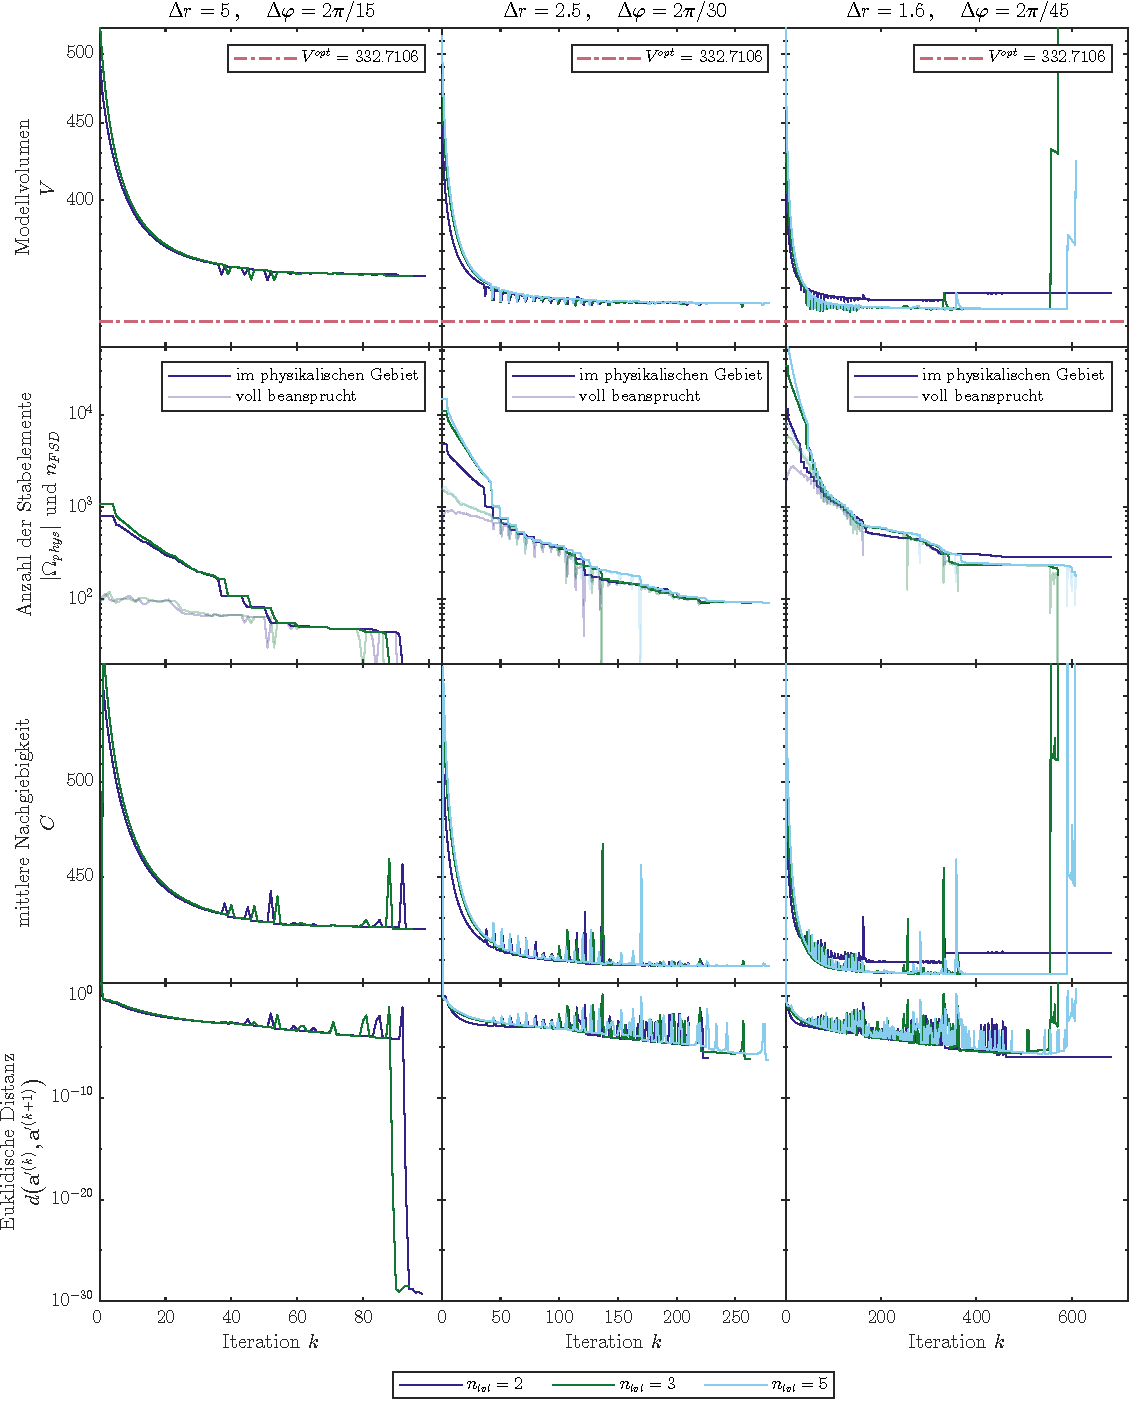
\includegraphics[scale=1]{results/michellCircCantilever/michellCircCantilever_optVal}};
		\node at (15, 9) {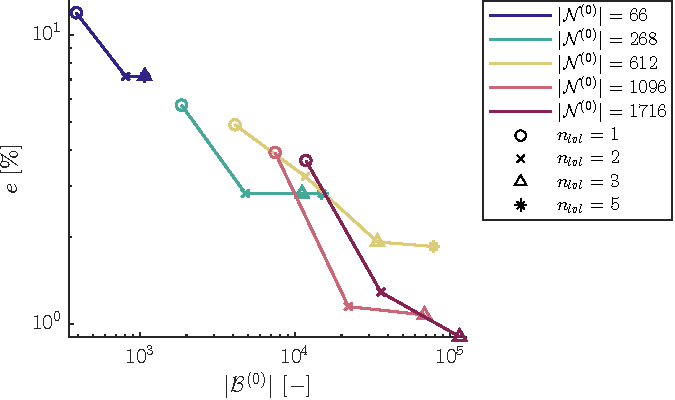
\includegraphics[scale=.75]{results/michellCircCantilever/michellCircCantilever_error_over_elements}};
		\node at (14, 3) {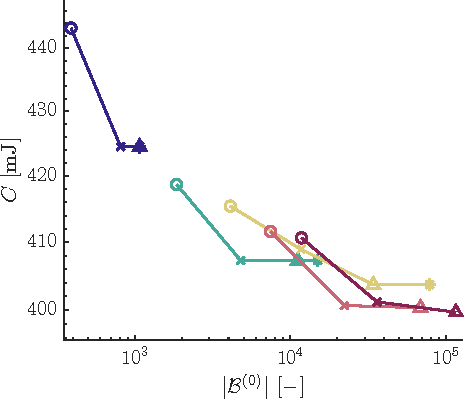
\includegraphics[scale=.75]{results/michellCircCantilever/michellCircCantilever_compliance_over_elements}};
		\node at (14.5, -3) {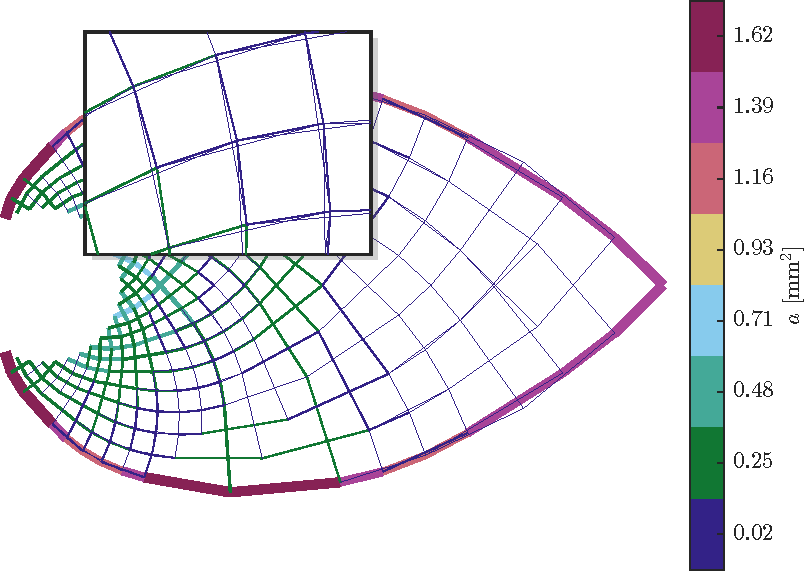
\includegraphics[scale=.55]{results/michellCircCantilever/michellCircCantilever_csaMagnified}};
		\node at (14, -9) {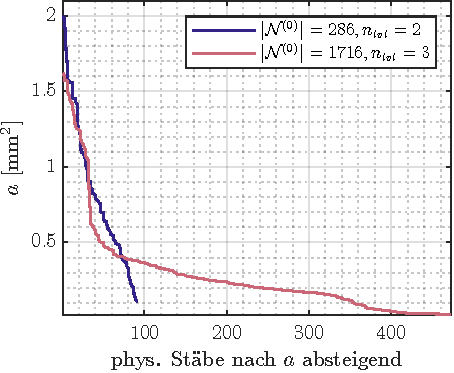
\includegraphics[scale=.85]{results/michellCircCantilever/michellCircCantilever_csaModelDistribution}};
		\node at (-6, -15) {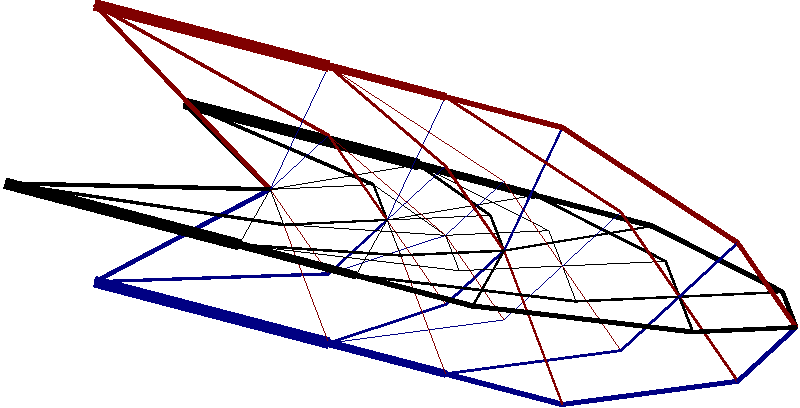
\includegraphics[scale=.6]{results/rectCantileverMultiLoad3D/vis/shown_under_vertical_load/trussModel_rectCantileverMultiLoad3D_lvl5_dx5.0}};
		\node at (4, -15) {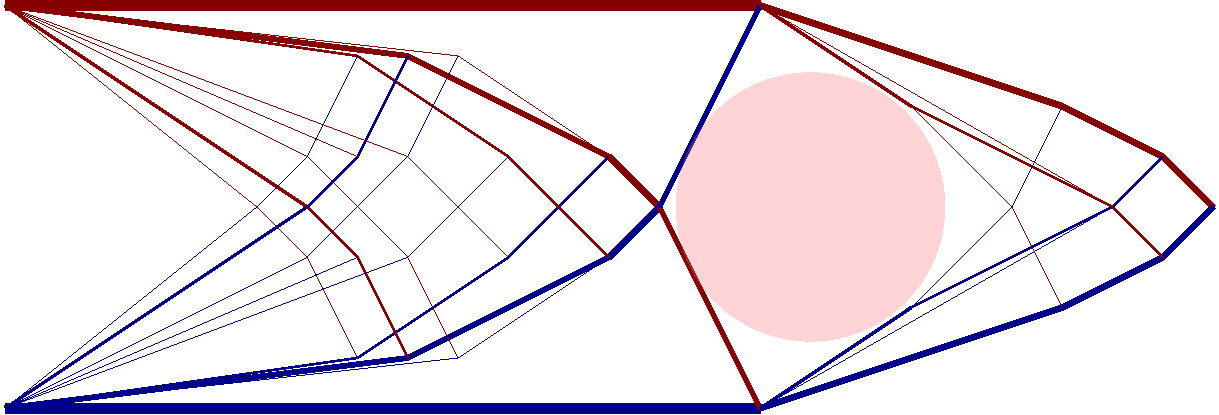
\includegraphics[scale=.5]{results/rectCantileverCircVoid/vis/trussModel_rectCantileverCircVoid_lvl8_dx2.5}};
		\node at (14, -15) {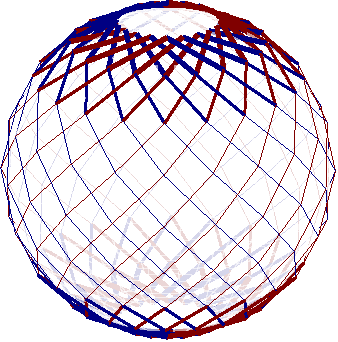
\includegraphics[scale=.9]{results/michellTorsionBall/vis/front/trussModel_michellTorsionBall_lvl3_dx0.0}};
	\end{tikzpicture}
	
\end{document}

